\documentclass{beamer}
\usepackage{listings}
\lstset{
%language=C,
frame=single, 
breaklines=true,
columns=fullflexible
}
\usepackage{subcaption}
\usepackage{url}


\usepackage{tikz}
\usetikzlibrary{arrows.meta,positioning}
\usepackage{pgfplots}
\pgfplotsset{compat=1.17}
\usepackage{tkz-fct}
\usepackage{mathrsfs}
\usepackage{txfonts}
\usepackage{tkz-euclide} 
\usetikzlibrary{calc,math}
\usepackage{float}
\newcommand\norm[1]{\left\lVert#1\right\rVert}
\renewcommand{\vec}[1]{\mathbf{#1}}
\providecommand{\pr}[1]{\ensuremath{\Pr\left(#1\right)}}
\usepackage[export]{adjustbox}
\usepackage[utf8]{inputenc}
\usepackage{amsmath}
\usetheme{Boadilla}



\title{Research Paper Presentation}
\author{Lanka Prasannna}
\date{CS20BTECH11029}
\begin{document}
%
\begin{frame}
\titlepage
\end{frame}
%slide 2
\begin{frame}
\begin{block}{Topic}
GAN-based Gaussian Mixture Model Responsibility Learning
\end{block}
\begin{block}{Authors}
\begin{enumerate}[]
\item Wanming Huang 
\item Richard Yi Da Xu
\item Shuai Jiang
\item Xuan Liang
\item Ian Oppermann

\end{enumerate}
\end{block}
\begin{block}{Year of Publication}
   2021.
\end{block}
\end{frame}



\begin{frame}
\begin{block}{Abstract}
\begin{enumerate}[]
\item Mixture model (MM) -dataset containing $K$ different modes. When each of the modes is associated with a Gaussian distribution, we refer to it as Gaussian MM or GMM. 
\item Modern large datasets- GMM unable to apply to compute conditional likelihood and responsibility probability.
\item We utilize the generative adversarial network (GAN) and we compute them at the data’s latent space $z$ instead of $x$.
\item However, this process of $z \rightarrow x$ is irreversible under GAN which
renders $\pr{k|x,\theta}$ infeasible.
\item Our paper proposed a novel method to solve it by using posterior consistency module (PCM).
\item PCM acts like a GAN, except its generator does not output the data, but
instead it outputs a distribution to approximate $\pr{k|x,\theta}$.
\end{enumerate}
 \end{block}
\end{frame}








\begin{frame}{Introduction}
Gaussian mixture model (GMM) assumes that all data points come from a mixture of a finite number of Gaussian distributions. The density function of the GMM is defined below
\begin{align}
    \pr{X=x}=\sum_{k=1}^{K}\alpha_{k}N(x;u_{k},\Sigma_{k})
\end{align}
where $K$ is the total number of Gaussians in the mixture, and $k^{th}$ component is characterized by a Gaussian distribution with weight $\alpha_{k}$ , mean $u_k$ and covariance matrix $\Sigma_{k}.$

\end{frame}


\begin{frame}{Introduction}
When Euclidean distance can be meaningfully defined over the data $x$ when it has a low dimensionality, one can compute both $\pr{x|k,\theta}$ and $\pr{k|x,\theta}$ directly, see Figure a. However, it will be difficult to do
so when dealing with complex and high data dimensional
data, such as images, shown in Figure b.

\begin{figure}[!tbp]
  \centering
  \subfloat[Low dimensional data]{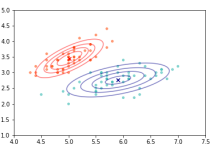
\includegraphics[width=0.4\textwidth]{1a.PNG}\label{fig:1a}}
  \hfill
  \subfloat[High dimensional data]{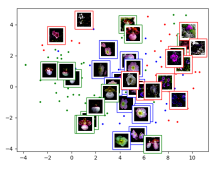
\includegraphics[width=0.4\textwidth]{1b.PNG}\label{fig:1b}}
  \caption{ Illustration of clustering}
\end{figure}
\end{frame}



\begin{frame}{Introduction}
\textbf{A. Posterior Consistency Module (PCM)}
\begin{enumerate}[]
\item PCM has allowed us to efficiently changing $\pr{z}$ in
GAN from single to a mixture of Gaussian densities while still be able to compute the responsibility $\pr{k|x,\theta}$.
\item Functions by assuming $\pr{k|x,\theta}$ to have an equivprobability latent counterpart $\pr{k|z,\theta}$. It is straightforward to compute $\pr{k|z,\theta}$ analytically:
\begin{align}
    \pr{k|z,\theta}=w \equiv (w_1,w_2,\cdots,w_K)=\\
    \left( \frac{\mathcal{N}(z|\mu_1,\sigma_1)}{\sum_{k=1}^{K}\mathcal{N}(z|\mu_k,\sigma_k)},\cdots,
    \frac{\mathcal{N}(z|\mu_K,\sigma_K)}{\sum_{k=1}^{K}\mathcal{N}(z|\mu_k,\sigma_k)}\right)
\end{align}
\item The same cannot be achieved by substituting $z$ with $x$. Therefore, we applied a neural network $C_{\theta}(x)$ with softmax output $\hat{w} = (\hat{w_1},\cdots,\hat{w_K})$. $\hat{w}$ is then compared with $w$ for consistency
\end{enumerate}
\end{frame}

\begin{frame}{Introduction}
\textbf{B. Closely related works}
\begin{enumerate}
\item Probabilistic GAN (PGAN) 
\item GM-GAN
\item GMVAE
\item VaDE
\item AAE
\item ClutsterGAN
\item VAE
\end{enumerate}
\end{frame}


\begin{frame}{Architecture}
The proposed architecture consists of three networks:
\begin{enumerate}
\item PCM as well as the loss function that matches it with $\pr{k|z,\theta}$.
\item A generator G which produces synthetic samples from GMM random vectors.
\item A discriminator D which encodes samples to feature vectors and discriminates between real and synthetic samples. 
\end{enumerate}
\begin{figure}[!tbp]
  \centering
  {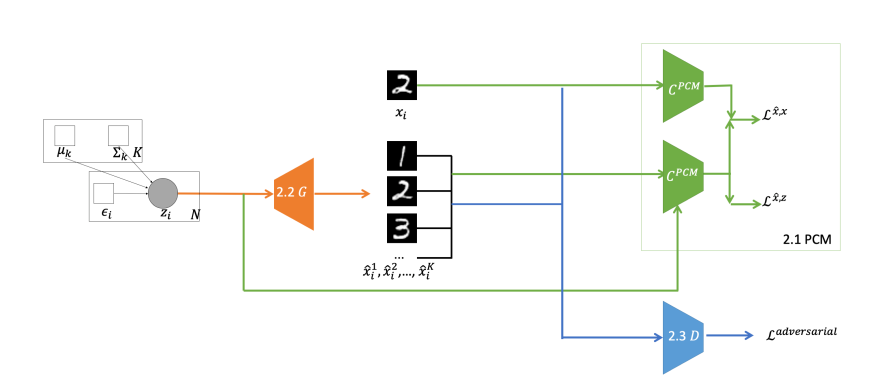
\includegraphics[width=0.8\textwidth]{2.PNG}\label{fig:2}}
  \hfill
  
  \caption{ The overall architecture. The feed-forward logic of the classifier C, the generator G and the discriminator D are marked with different colours.}
\end{figure}

\end{frame}


\begin{frame}{Architecture}
\textbf{A. PCM}\\
The PCM is comprised of a classifier/ generator $C_{PCM}$ which outputs $\pr{k|z,\theta}$ given $x$. When a synthetic data $\hat{x}$ is used as its input, the output approximates $\pr{k|\hat{x},\theta}$ 
and it needs to be matched against:

1. $\pr{k|z,\theta}$, this is to ensure that the responsibility
probability condition on its latent variable $z$ is similar to the responsibility distribution dependent on $x$. The corresponding loss is named as:
\begin{figure}[!tbp]
  \centering
  {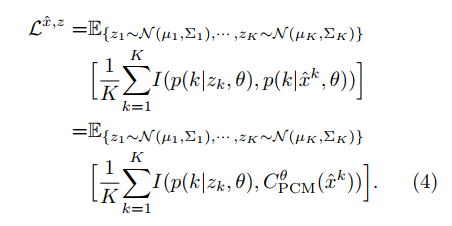
\includegraphics[width=0.6\textwidth]{equation1.PNG}}
  \hfill
\end{figure}
\end{frame}



\begin{frame}{Architecture}
2. $\pr{k|x,\theta}$, this is to ensure that the distribution generated is similar to those generated by the real data $x$. The corresponding loss is named as:
\begin{figure}[!tbp]
  \centering
  {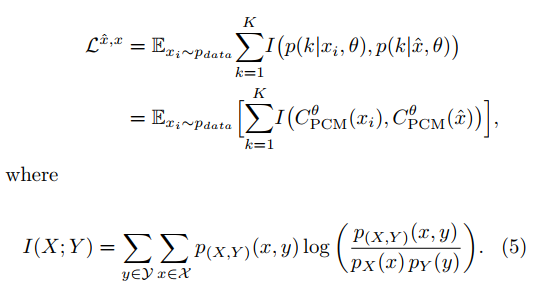
\includegraphics[width=0.8\textwidth]{equation2.PNG}}
  \hfill
\end{figure}

\end{frame}




\begin{frame}{Architecture}
 \textbf{B. Generator\\} 
 \begin{enumerate}[]
 \item We sample one random vector from each Gaussian as $z_i = [z_{i}^{1},\cdots, z_{i}^{K}]$. These vectors are used to generate $K$ synthetic images $[\hat{x_i}^{1},\cdots,\hat{x_i}^{K} ]$. 
 \item The classification output is used to weigh the adversarial loss calculated from each pair of a generated sample $\hat{x_i}^{k}$ and the real image $x_i$.
 \item Our design expects the training to be performed in an ``end-to-end” fashion, the reparameterization trick is applied to the $z_i$ sampling process so that the backpropagation can be used to update the parameters $\mu_k$ and
$\Sigma_k$ of each Gaussian.
\item Instead of sampling $z_{i}^{k} \sim \mathcal{N}(\mu_k,\Sigma_k)$, we define $z_{i}^{k} = \Sigma_k\epsilon + \mu_k \forall k \in [1, K],$ where $\epsilon$ is sampled as $\epsilon \sim \mathcal{N}(0, I)$.
 \end{enumerate}
\end{frame}



\begin{frame}{Architecture}
\textbf{C. Discriminator\\}
The design of the discriminator has two options:
\begin{enumerate}
\item Whether the image encoding layers are shared with the classifier or not.
\item The image encoding network is followed by a standard linear logistic regression to identify the given image to be real or fake.
\end{enumerate}
The adversarial loss, which is calculated over K pairs
of real and synthetic samples as:
\begin{figure}[!tbp]
  \centering
  {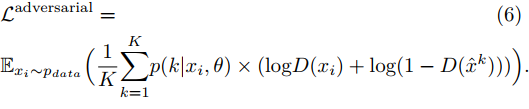
\includegraphics[width=0.8\textwidth]{equation4.PNG}}
  \hfill
\end{figure}
\end{frame}




\begin{frame}{Architecture}
\textbf{D. Training parameters for the prior distribution\\}
\begin{figure}[!tbp]
  \centering
  {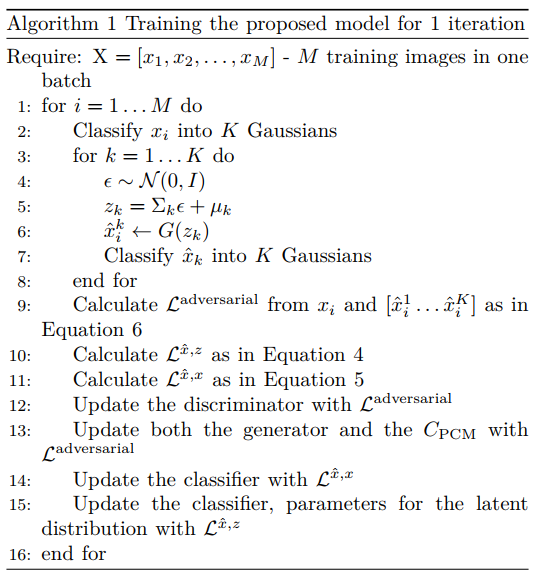
\includegraphics[width=0.6\textwidth]{algorithm.PNG}}
  \hfill
\end{figure}
\end{frame}



\begin{frame}{Experiments}
\textbf{A. Experiment setup\\}
The datasets we use are the MNIST, Fashion-MNIST and Oxford-102 Flower datasets. In particular, we only select a subset of Oxford-102 to perform the training, which is the images that belong to the first 10 classes. 
\end{frame}


\begin{frame}{Experiments}
\textbf{B. Linear Interpolation across Gaussian\\}
\begin{figure}[!tbp]
  \centering
  {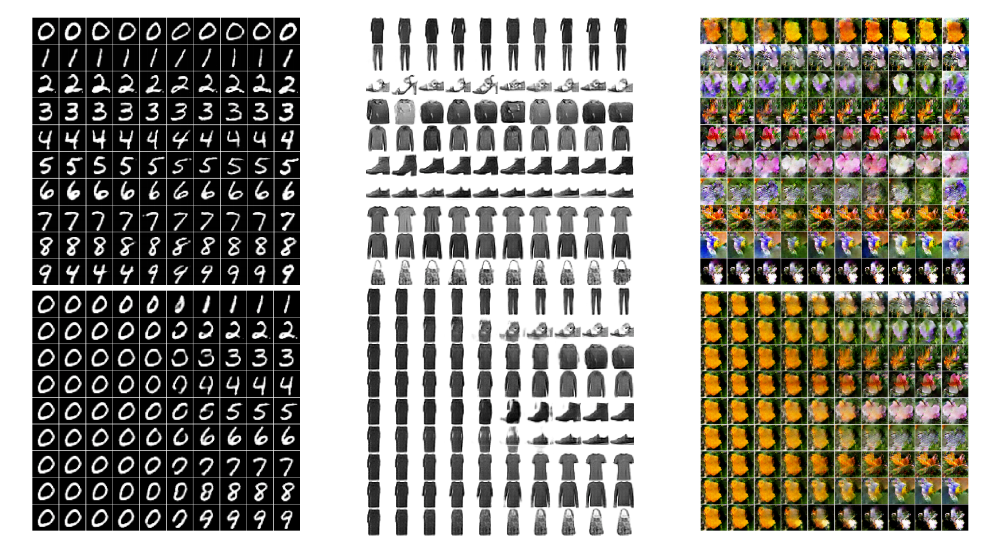
\includegraphics[width=0.7\textwidth]{fig-4.PNG}}
  \hfill
  
  \caption{Samples generated by the proposed models trained on the MNIST (left column), Fashion-MNIST (middle column) and CIFAR-10 (right column) datasets. The top row contains images generated using random vectors sampled from a different Gaussian. The bottom row shows the linear interpolation result from one Gaussian to another }
\end{figure}
\end{frame}



\begin{frame}{Experiments}.
\begin{enumerate}[]
\item  When we are performing the linear interpolation as in the right panels, the random vector $z$ for each image generation is calculated as $z = \Sigma_k\epsilon + \mu_k \forall k \in [1, K],$ where $\epsilon$ is sampled as $\epsilon \sim \mathcal{N}(0, I)$. $\epsilon$ is kept the same for all images for each dataset.
\item We can draw two conclusions from the results in above figure. First, a fully trained proposed method can learn to ``allocate” each class of image to a Gaussian.
\item Second, the trained model can be used to perform smooth linear interpolation between Gaussians and even among more than two Gaussians.
\end{enumerate}
\end{frame}



\begin{frame}{Experiments}

\begin{figure}[!tbp]
  \centering
  {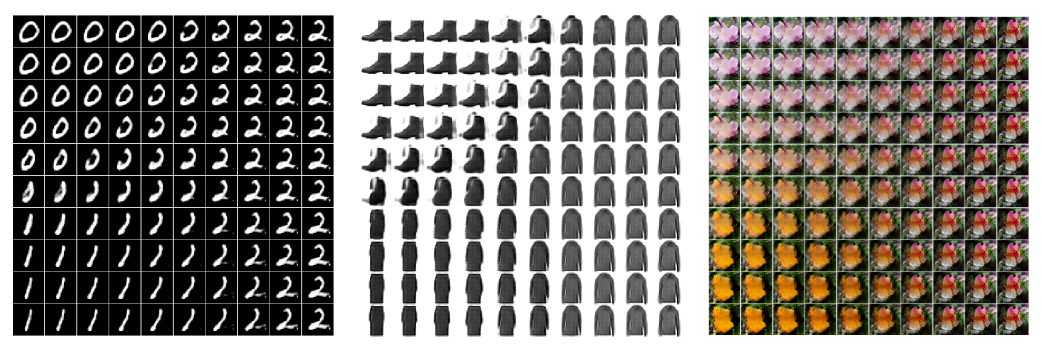
\includegraphics[width=0.8\textwidth]{fig-3.PNG}}
  \hfill
  
  \caption{Linear interpolation over 3 Gaussians on the MNIST, Fashion-MNIST and Oxford-102 dataset}
\end{figure}
\end{frame}



\begin{frame}{Experiments}
 \textbf{C. Image Generation Quality\\} 
 The generation performance is measured with two
commonly used metrics: Inception score and Fréchet Inception Distance (FID) score.
\begin{enumerate}
 \item Inception score is calculated as $I = exp(E_x D_{KL}(p(y|x)||p(y)))$, and a higher value generally indicates a better performance, where $x$
is a generated image and $y$ is the label predicted by
the Inception model
\item FID score: lower value shows a better image quality and diversity. It calculates the difference between real images $x$ and generated images
$g$ as $FID_{(x, g)} = ||\mu_x - \mu_g||^2_{2} + Tr(\Sigma_x + \Sigma_g - 2(\Sigma_x\Sigma_g)^\frac{1}{2} )$.
\end{enumerate}
\end{frame}



\begin{frame}{Experiments}
\begin{figure}[!tbp]
  \centering
  {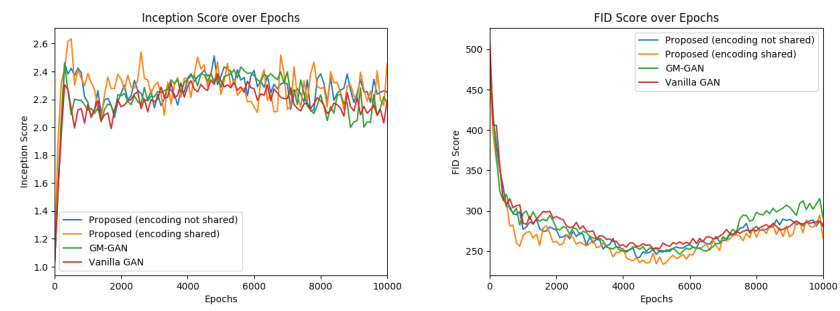
\includegraphics[width=0.8\textwidth]{fig-5.PNG}}
  \hfill
  
  \caption{Inception score and FID score over training epochs on the Oxford dataset}
\end{figure}
From the above figure, it is clear to see that the proposed method is able to out-perform previous baseline models in terms of image generation quality. The
shared feature encoding layers would further improve the performance and reduce the size of the network.
\end{frame}



\begin{frame}{Experiments}
 \textbf{D. Network Compression\\} 
Applying Gaussian mixture to GANs can significantly reduce the number of
parameters while achieving close performance compared with the vanilla GAN.
\begin{figure}[!tbp]
  \centering
  {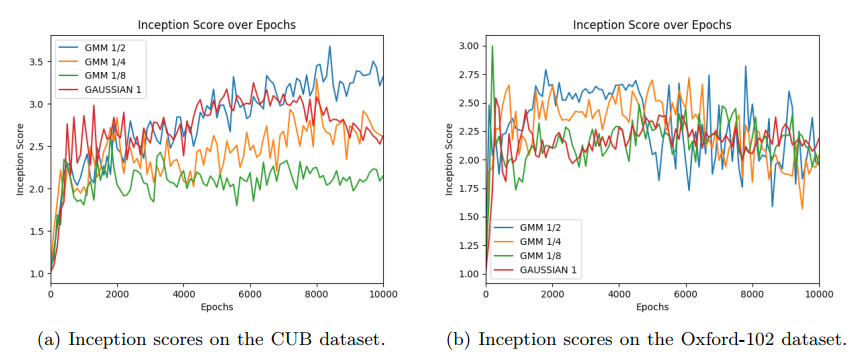
\includegraphics[width=0.8\textwidth]{fig-6.PNG}}
  \hfill
  
  \caption{Inception scores over epochs for the proposed GMM-based GAN with various size of the network and the vanilla GAN.}
\end{figure}
\end{frame}



\begin{frame}{Experiments}
 \textbf{E. Performance on Highly Imbalanced Dataset\\}   
 We also demonstrate the performance on the highly imbalanced dataset.
 \begin{figure}[!tbp]
  \centering
  {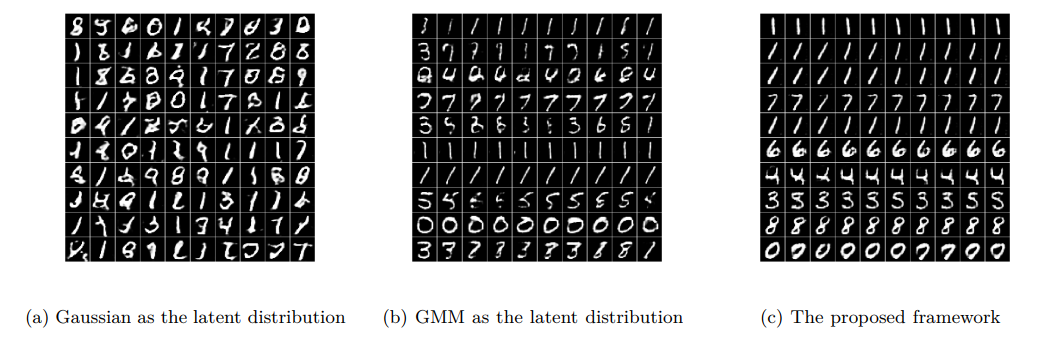
\includegraphics[width=1.0\textwidth]{fig-7.PNG}}
  \hfill
  
  \caption{Performance on high imbalanced dataset.}
\end{figure}
\end{frame}


\begin{frame}{Experiments}
\begin{enumerate}[]
  \item The imbalanced dataset we used is a subset of the original MNIST dataset. From digit 0 to digit 9, we randomly choose digit d as the dominant category. 1000 samples are randomly selected from all other categories and the category $d$ is kept the same. This becomes the imbalanced training dataset.
  \item While using both the standard Gaussian and GMM result in poor generation quality and collapsed output, the proposed framework is able to deliver digits with clear shape and categorization.
\end{enumerate}
\end{frame}



\begin{frame}{Conclusion}
  In addition to GMM modelling, we also demonstrate the multitude of benefits in
our approach: 
\begin{enumerate}
   \item We demonstrated through experiments that our proposed method retains GAN’s ability in sharper image generation compared with other GMM GAN methods.
   \item The proposed approach can significantly save the computation cost as only half number of parameters is required to achieve the same image generation quality compared to classic DCGAN.
   \item The proposed method surpasses previous baselines when dealing with highly imbalanced dataset.
\end{enumerate}
\end{frame}





\begin{frame}
   \centering
    \textcolor{blue}{\Huge{\textbf{THANK YOU}}}
\end{frame}

\end{document}